\section{Komponenten}

%5.1 Server Software
\subsection{Komponente \textit{ServerSoftware}}
\begin{figure}[H]
\centering
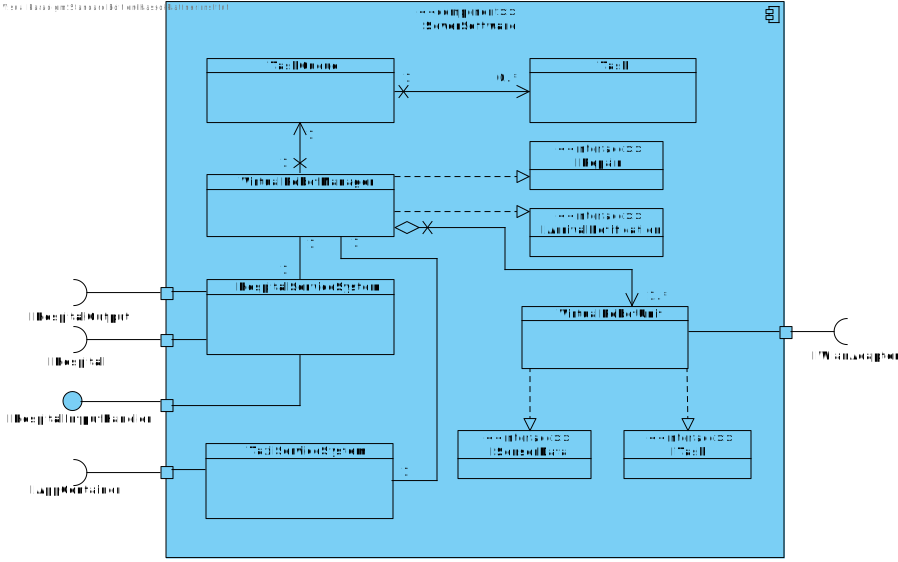
\includegraphics[height=0.7\textwidth, angle=90]{img/2-Entwurf-5-ServerSoftware}
\caption{\emph{ServerSoftware}-Komponentendiagramm}
\label{KomponentenStruktur1}
\end{figure}
Abbildung \ref{KomponentenStruktur1} zeigt ein Komponentendiagramm von \emph{ServerSoftware}. 
Diese Komponente umfasst sechs Klassen: \textit{TaskSystem}, \textit{Task}, \textit{VirtualRobotManager}, \textit{VirtualRobotUnit}, \textit{HospitalServiceSystem} und \textit{TaxiServiceSystem}.

Die Klasse \textit{Task} beinhaltet die Aufgaben, die von der \textit{TaskPriorityQueue} verwaltet werden. 
Die \textit{TaskPriorityQueue} priorisiert die \textit{Tasks} und ordnet diese so an, dass der \textit{VirtualRobotManager} die \textit{Task} mit der höchsten Priorität erhält. 
Der \textit{VirtualRobotManager} ist die zentrale Kommunikationskomponente in der \textit{ServerSoftware}, der für die Koordination der \textit{RobotUnits} zuständig ist, wobei die \textit{RobotUnits} serverintern als \textit{VirtualRobotUnits} repräsentiert werden, um RPC zu ermöglichen. Über das \textit{HospitalServiceSystem} und das \textit{TaxiServiceSystem} werden \textit{Orders} entgegengenommen. Daraus erzeugt der \textit{VirtualRobotManager} \textit{Tasks}. Der \textit{VirtualRobotManager} deligiert die \textit{Tasks} entweder sofort an eine verfügbare \textit{RobotUnit} oder speichert diese, falls keine \textit{RobotUnit} verfügbar ist, in der \textit{TaskPriorityQueue}. Die am besten geeignete \textit{RobotUnit} wird anhand der Sensordaten ermittelt, die über das Interface \textit{ISensorData} bereitgestellt werden. Die \textit{Task} wird anschließend über das Interface \textit{ITask} der \textit{RobotUnit} zugewiesen. Des Weiteren implementiert der \textit{VirtualRobotManager} die Interfaces \textit{IRepair} und \textit{IArrivalNotification}, womit die \textit{RobotUnits} in der Lage sind, einen Defekt und Ihre Ankunft an einer \textit{Destination} zu melden.
%5.1 Robot Software
\subsection{Komponente \textit{RobotSoftware}}
\begin{figure}[H]
\centering
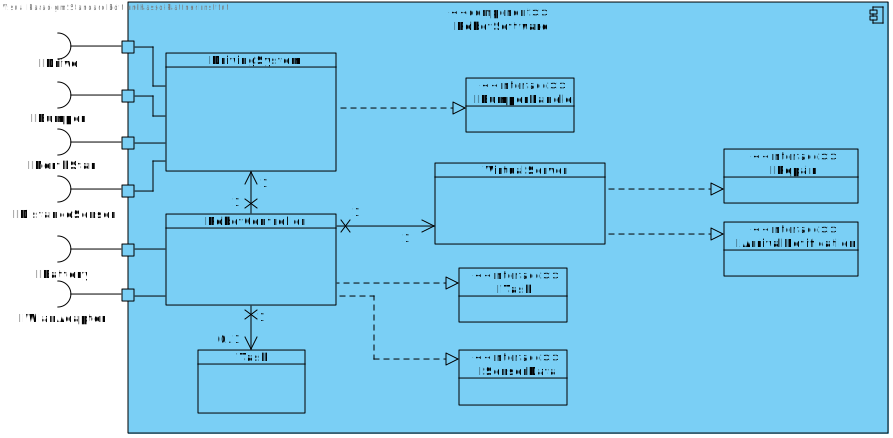
\includegraphics[width=1\textwidth]{img/2-Entwurf-5-RobotSoftware}
\caption{\emph{RobotSoftware}-Komponentendiagramm}
\label{KomponentenStruktur2}
\end{figure}
In Abbildung \ref{KomponentenStruktur2} ist das Komponentendiagramm der Komponente \textit{RobotSoftware} dargestellt. 
Die Komponente enthält drei Klassen: \textit{DrivingSystem}, \textit{RobotController} und \textit{Task}.


Das \textit{DrivingSystem} stellt eine Abstraktion der Hardware dar und wird dazu genutzt, Ziele anzufahren und dabei,
falls nötig, Hindernisse zu umfahren. 
Dazu greift es auf die von der Hardware bereitgestellten Interfaces zurück.
Um auf Kollisionen reagieren zu können, implementiert das \textit{DrivingSystem} die Schnittstelle \textit{IBumperHandler}.
Der \textit{RobotController} stellt dem Server das Interfaces \textit{ISensorData} zur Verfügung und verwaltet den gerade
zu absolvierenden \emph{Task}. 
Zur Messwertübermittlung greift er zum einen auf das \textit{DrivingSystem} und zum anderen auf das
von der Hardware angebotenen Interface \textit{IBattery} zu.
